%%%%%%%%%%%%%%%%%%%%%%%%%%%%%%%%%%%%%%%%%%%%%%%%%%%%%%%%%%%%%%%%%%%%%%%%%%%%
%%%%%                          ANNEXE 1                               %%%%%%
%%%%%%%%%%%%%%%%%%%%%%%%%%%%%%%%%%%%%%%%%%%%%%%%%%%%%%%%%%%%%%%%%%%%%%%%%%%%

\appendix
\renewcommand\chaptername{Annexe~}
% \phantomsection

\lhead[\fancyplain{}{\leftmark}]%Pour les pages paires \bfseries
      {\fancyplain{}{}} %Pour les pages impaires
\chead[\fancyplain{}{}]%
      {\fancyplain{}{}}
\rhead[\fancyplain{}{}]%Pour les pages paires 
      {\fancyplain{}{\rightmark}}%Pour les pages impaires \bfseries
\lfoot[\fancyplain{}{}]%
      {\fancyplain{}{}}
\cfoot[\fancyplain{}{\thepage}]%\bfseries
      {\fancyplain{}{\thepage}} %\bfseries
\rfoot[\fancyplain{}{}]%
     {\fancyplain{}{\scriptsize}}


%%%%%%%%%%%%%%%%%%%%%%%%%%%%%%%%%%%%%%%%%%%%%%%%%%%%%%%%%%%%%%%%%%%%%%%%%%
%%%%%                      Start part here                          %%%%%%
%%%%%%%%%%%%%%%%%%%%%%%%%%%%%%%%%%%%%%%%%%%%%%%%%%%%%%%%%%%%%%%%%%%%%%%%%%

\chapter{Annexe 1 : Maîtrise du procédé d'injection-moulage des thermoplastiques}
\label{Ann:process_control}

%==============================================================================	Résumé du chapitre

\begin{center}
\rule{0.7\linewidth}{.5pt}
\begin{minipage}{0.7\linewidth}
\smallskip

\textit{
Cette annexe propose une étude bibliographique de la maîtrise du procédé d'injection-moulage des thermoplastiques, de 1975 à 2015.
}

%\smallskip
\end{minipage}
\smallskip
\rule{0.7\linewidth}{.5pt}
\end{center}

%\adjustmtc
\minitoc
% \newpage
\bigskip

Cette annexe est complémentaire de la Section \ref{subsec:process_control} "Maîtrise du procédé d'injection-moulage des thermoplastiques" du Chapitre \ref{ch:objectives}.
L'objectif de la maîtrise d'un procédé est de maîtriser la qualité du produit : c'est à dire de limiter la dispersion des caractéristiques des pièces.
Il s'agit en priorité d'effectuer des mesures pertinentes sur l'état du procédé, puis de les analyser afin de détecter les dérives.
Une dernière étape est l'ajustement automatique des paramètres du procédé.

\begin{figure}[hbtp]
	\centering
	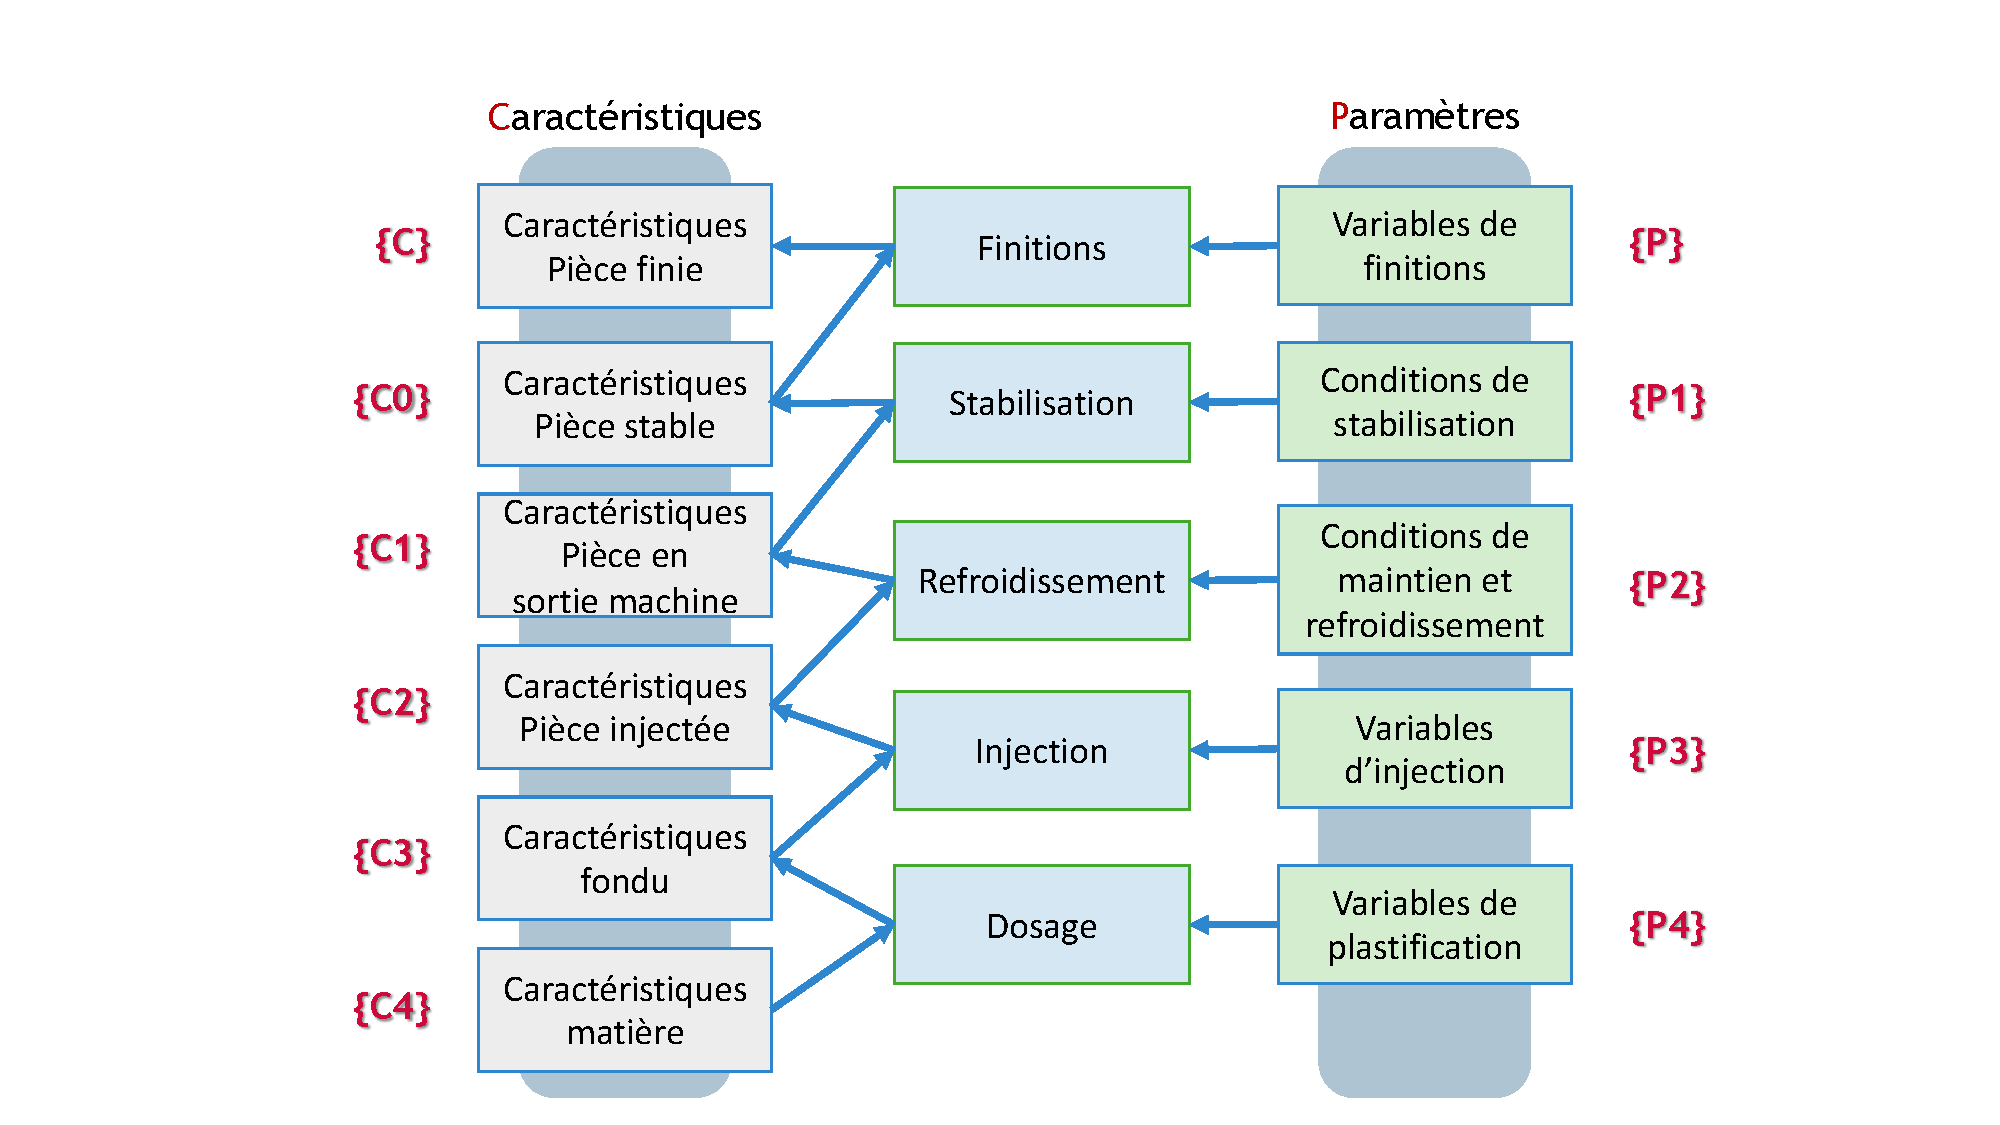
\includegraphics[width=0.80\textwidth,height=\textheight,keepaspectratio]{../Chap1/Figures/Sapristi_ZigZag.pdf}
	\caption{Représentation \textit{Zig Zag} du procédé d'injection-moulage des thermoplastiques.}
	\label{fig:annexe_zigzag}
\end{figure}

La maîtrise d'un procédé de production peut être discrétisée en différentes étapes :
\begin{enumerate}
	\item réglage initial d'un point de fonctionnement (paramètres $\boldsymbol{P}_{2-4}$) : connaissance humaine et système expert,
	\item régulation du point de fonctionnement $\boldsymbol{C}_{2-3}$ : automatique et contrôle adaptatif,
	\item détection des dérives du procédé $\boldsymbol{C}_{1-3}$,
	\item ajustement des paramètres $\boldsymbol{P}_{2-4}$ afin de modifier les caractéristiques $\boldsymbol{C}_{0-1}$.
\end{enumerate}
\noindent
Nous indiquerons à quelle phase de notre représentation \textit{Zig-Zag}, voir la Figure \ref{fig:annexe_zigzag}, s'intéresse les différents travaux étudiés dans notre revue.

\section{Réglage initial du point de fonctionnement}
La pratique industrielle du procédé d'injection-moulage fait appelle au savoir-faire du technicien pour régler le point de fonctionnement initial.
Les valeurs des caractéristiques du produit sont fonction d'un point de fonctionnement du procédé.
De plus, le procédé d'injection-moulage n'est pas bijectif : il existe plusieurs points de fonctionnement différents pour des caractéristiques de produit identiques.
L’approche classique de réglage employée par le technicien régleur est l’essai-erreur.
Aussi, lors du démarrage du procédé, les premiers cycles de la production sont dédiés au réglage initial.
Des échantillons sont pris quelques secondes après leurs sorties du moule et leurs qualités est rapidement évaluée par observation visuelle.
Dans un premier temps, il s'agit de contrôle l'absence de manque de matière (trous dans la pièce), puis les déformations géométriques importantes et enfin les traces de brûlures et givrages.
L’opérateur utilise ensuite ses connaissances pour améliorer les réglages et respecter le cahier des charges : cotations géométriques précises, défauts d'aspect, caractéristiques mécaniques.
Sur les pièces les plus techniques, des mesures géométriques sont effectuées à l'aide d'un moyen de mesure manuel, comme un pied à coulisse ou un comparateur.

En 2009, \citeauthor{richard_analyse_2009} analysèrent les stratégies employées par des techniciens-régleurs plasturgistes \cite{richard_analyse_2009}.
Les observations furent recueillies sur un intervalle de dix années par \citeauthor{pastre_role_2004} \cite{pastre_role_1994, pastre_role_2004} auprès de 13 régleurs d’une entreprise de fabrication de produits, dont la qualité de finition est élevée \cite{pastre_role_1994, pastre_role_2004}.
Leurs niveaux de compétences et leurs parcours professionnels sont variés.
Certains ont une formation technique, mais la majorité a appris par la pratique, sans formation initiale.
6 paramètres du procédé sont ajustables de manière binaire : augmenter ou diminuer la valeur de réglage ; la température de la matière fondue ($\boldsymbol{P}_4$ Figure \ref{fig:annexe_zigzag}), la durée d'injection $\boldsymbol{P}_3$, la contre-pression $\boldsymbol{P}_{2-3}$, la pression de commutation $\boldsymbol{P}_3$, le niveau de pression qui déclenche le passage de la phase d'injection à celle de maintien $\boldsymbol{P}_{2-3}$, la pression de maintien $\boldsymbol{P}_2$, la durée de maintien $\boldsymbol{P}_2$, la durée de refroidissement $\boldsymbol{P}_2$,
Un septième paramètre concerne le changement de la buse.
Les auteurs identifient les deux sources d'informations qui sont utilisés par les régleurs : l'observation de la courbe de la pression d'injection pendant le cycle d'injection et la présence d'un défaut sur la pièce.
L'étude est une simulation visant à évaluer la méthode de résolution de problèmes des régleurs, aussi elle se limite aux seules défauts de manque de matière, retrait, retassure ou brûlure.
Le profil de la courbe de la pression d'injection est utilisée par les techniciens-régleurs pour déduire les caractéristiques des phases d'injection, de maintien et de refroidissement ($\boldsymbol{C_2-3}$).
% C'est un outil qui semble permettre de diagnostiquer la cause d'un défaut.
L'étude évalue la réaction des techniciens-régleurs à 17 situations différentes : lorsque les défauts sont visibles sur la pièce, ou lorsque la présence du défaut est déductible à partir de la courbe.
Certains techniciens-régleurs réalisent le réglage des paramètres sans étudier la courbe.
Deux techniciens-régleurs sur le panel de huit obtiennent des résultats plus élevées que les autres car ils étudient systématiquement la courbe de pression d'injection ; de plus l'étude montre qu'ils ont une stratégie de réglage répétable.
Les six techniciens-régleurs restant n'étudient pas ou analysent mal la courbe ; l'étude montre qu'ils n'ont pas de stratégie de réglage.
Les résultats de cette étude montrèrent que la cause principale des différences de réaction entre régleurs est liée à la difficulté de lecture de cette courbe.  % \textemdash la dispersion de réglages \textemdash 
En revanche, les causes de chacun des défauts sont connues de l’ensemble des régleurs formés ou non.
Nous tirons de cette étude quatre informations à propos de la méthode de détermination du point de fonctionnement :
\begin{itemize}
	\item les techniciens-régleurs ont appris par la pratique les relations entre les défauts et leurs causes,
	\item les techniciens-régleurs observent la pièce pour déterminer la présence de défauts,
	\item l'analyse du profil de la pression d'injection permet de mieux régler.
\end{itemize}
Néanmoins, il existe de nombreuses autres caractéristiques qui peuvent être analysées, en particulier l'évolution de la température et la pression dans le moule.
De plus, le panel (8) de cette est faible, ainsi que le nombre de situations évaluées (17).
Suite à cette étude, nous remarquons que des systèmes d'assistance au réglage sont aujourd'hui déployés dans l'industrie.
Ils proposent de calculer des indicateurs de l’état du procédé, ce qui permet d'éviter les difficultés de lecture de la courbe de pression, mais également des nombreuses autres caractéristiques du procédé qui sont difficile à interpréter.

\subsection{Apport des systèmes experts} \label{subsubsec:initial_expert}
Dans la littérature, des systèmes experts ont été utilisés pour choisir des paramètres initiaux, afin de produire des pièces plus rapidement, lors d'une mise en place d'une production.
Un système expert s’appuit sur une base de connaissances : un ensemble de relations causales pondérées, qui a été construit à partir des connaissances humaines et des connaissances théoriques du procédé.
La base de connaissance représente souvent des règles empiriques.
Un moteur d'inférence applique des règles logiques à partir des connaissances et en déduit de nouvelles connaissances, ce qui permet de répondre afin de choisir des paramètres.

Les performances de ces systèmes sont parfois validées par des simulations numériques \cite{jan_expert_1992}.
En 1993, \citeauthor{kameoka_development_1993} vérifièrent que le système expert est capable de proposer des réglages identiques à ceux d’un technicien-régleur de niveau moyen \cite{kameoka_development_1993}.
Des systèmes hybrides peuvent être constitués de règles empiriques et de cas d'applications spécifiques \cite{shelesh-nezhad_intelligent_1997}.
Ces systèmes simulent une démarche de réglage humaine basée sur la connaissance de relations linéaires simples entre les paramètres du procédé.
\citeauthor{bozdana_development_2002} proposèrent une base de connaissances de 623 presses à injecter et 27 matériaux différents \cite{bozdana_development_2002}.
Ce système expert permet de sélectionner le couple machine-matériau le plus approprié, pour une pièce donnée.

\section{Régulation du point de fonctionnement} \label{subsec:regulation}
Diminuer la dispersion d’un procédé de production permet de limiter les rebuts.
Pour cela, il est nécessaire de maîtriser le procédé.
Il est possible d’asservir les paramètres réglables pour garantir que le procédé reste sur le point de fonctionnement défini.
Cependant, asservir un procédé non linéaire aux multiples commandes et sorties est compliqué.
La littérature de la théorie du contrôle automatique propose de nombreux travaux appliqués aux productions industrielles.
Les recherches aboutissent souvent à des solutions commerciales.
Dans ce domaine d'étude, nous notons le dynamisme du secteur de la chimie de synthèse.
La régulation du procédé s'appuie sur l'analyse de la transformation de la matière, qui change d'état au court du cycle.
Les contraintes qui lui sont appliquées pendant le cycle conditionnent son état final.
Le produit final correspond à la pièce sortie de la machine, après une durée de stabilisation, durant laquelle des modifications géométriques peuvent se produire (par exemple des déformations liées aux contraintes internes qui se relâchent).
Les premiers développements ont porté sur la régulation de paramètre unique.

\subsection{Utilisation de l'automatique} \label{subsubsec:automatic}
Dès 1975, un asservissement a été breveté par \citeauthor{laczko_controller_1975}, sous la forme d'une consigne sur la viscosité de la matière \cite{laczko_controller_1975}.
La pression mesurée dans l'outillage permet de réguler la pression hydraulique qui est appliquée pendant le cycle d'injection, afin de garantir une consigne sur la viscosité de la matière.
Cette asservissement est hydraulique et ne nécessite pas de micro-contrôleur.

%\paragraph{Régulation de la pression dans l'outillage}\mbox{} \\
% \citeauthor{maitre_sur_1997} montrent que la position du front du polymère fondu est régi par une équation en pression à double non linéarité \cite{maitre_sur_1997}.
Dans la littérature, la caractéristique la plus étudiée est la masse de la pièce ($\boldsymbol{C_0}$ Figure \ref{fig:annexe_zigzag}).
Le paramètre du procédé qui est le plus étudié pour la régulation est la pression dans l'outillage \cite{fara_evaluation_1985, kamal_dynamics_1987} ($\boldsymbol{P_3}$ Figure \ref{fig:annexe_zigzag}).
Sur ce sujet, \citeauthor{fara_control_1988} a évalué l'utilisation des régulateurs Proportionnel Intégrateur et Proportionnel Intégrateur Dérivateur \cite{fara_control_1988}.
Dans son travail de doctorat, le système hydraulique du vérin d’injection de la presse a été modifié pour inclure deux servovalves, afin de piloter la pression d’injection.
Cela permet d’asservir la pression qui est mesurée directement dans le moule à une consigne.
% Il obtient une meilleure réponse pour la pression hydraulique par PI, pour la pression dans la buse par PID, et pour la pression dans le moule par PI ou PID.
Les valeurs des correcteurs Proportionnel, Intégrateur et Dérivateur ont été choisies à partir de simulations.
Les expérimentations montrèrent que la valeur de la pression dans l'outillage a un comportement non linéaire.
La régulation a été effectuée à l'aide d'un gain échelonné sur la servovalve, selon la valeur de la pression.
Ce procédé de régulation provoque néanmoins des oscillations de pression à la fin de la phase d'injection, car la commande de la valve est binaire.

En 1987, \citeauthor{agrawal_injection-molding_1987} \cite{agrawal_injection-molding_1987} a réalisé un état de l'art du contrôle du procédé d’injection-moulage, dans lequel ils indiquent que les régulateurs Proportionnel Intégrateur (PI) et Proportionnel Intégrateur Dérivateur (PID) sont difficilement utilisables.
En effet, les auteurs estiment que le procédé d'injection-moulage n'atteint jamais un régime permanent ; les paramètres du procédé doivent régulièrement être ajusté afin de compenser les dérives, c'est pourquoi les coefficients des régulateurs PI et PID devraient être ajustés régulièrement.
Ils concluent sur l’intérêt des contrôleurs autorégulateurs, contrôleurs optimaux et contrôleurs prédictifs.
Cependant, ces contrôleurs ne réagissent qu’à une unique variable du procédé ; alors que le procédé d'injection-moulage à des interactions multivariées.
Nous remarquons que les contrôleurs uni-variés entrainent un risque pour la robustesse de la régulation, car ils ne prennent pas en compte les interactions entre les paramètres.
% C'est pourquoi, ils peuvent avoir l'effet opposé de celui souhaité.
Le risque est de dérégler le procédé.
Le contrôleur uni-varié peut appliquer une correction idéale pour une variable, mais cette correction sera erronée pour les autres variables, d'où l'effet opposée qui dérèglera le procédé.
Enfin, \citeauthor{agrawal_injection-molding_1987} défend l'idée que les caractéristiques de la matière fondue doivent être mesurées en direct, plutôt que de mesurer des variables de la machines ; cela permet de limiter les erreurs dû aux mesures indirectes.
% C'est le début de la mise en place de capteurs directement au contact de la matière, dans l'outillage.
Nous qualifions ces méthodes de mesure "invasives" pour le procédé.
Elles nécessitent une intégration compliquée au sein de l'outillage.
Nous discutons dans le Chapitre \ref{ch:measure} des différentes méthodes de mesures des variables du procédé et de la notion d'invasivité.

Par la suite, \citeauthor{fara_comprehensive_1990} ont développé une méthode de régulation de la pression dans le moule qui est capable de rejeter des perturbations externes, tel que la variation des propriétés du polymère et de la matière fondu ($\boldsymbol{P_1}$ et $\boldsymbol{P_2}$ Figure \ref{fig:annexe_zigzag}) \cite{fara_comprehensive_1990}.
L'étude ne s'intéresse qu'à la régulation de la pression dans le moule.
Les auteurs ont proposé comme perspective l'utilisation du contrôle multivarié et du contrôle adaptatif.

En 1995, \citeauthor{kazmer_dynamic_1995} a proposé le système \textit{Dynamic Feed Control} afin d'équilibrer le débit d'injection de la matière pour les moules multi-empreintes ($\boldsymbol{P_3}$ Figure \ref{fig:annexe_zigzag}) \cite{kazmer_dynamic_1995}.
Plusieurs valves permettent de réguler la pression dans chacune des empreintes, pendant l'injection.
Les résultats obtenus ont montré une réduction de 75\% de la variabilité de la masse des pièces produites.
La capabilité long terme (Ppk) du procédé est augmentée de 0,52 à 1,67.
Ce système demande un développement spécifique de l'outillage du moule.
Il est néanmoins très utilisé aujourd'hui dans l'industrie.

Des travaux se sont intéressés à la régulation de la température de la matière fondue ($\boldsymbol{P_4}$  Figure \ref{fig:annexe_zigzag}), par \citeauthor{kamal_injection_1986} \cite{kamal_injection_1986, gomes_injection_1986}, puis par \citeauthor{gustafson_model_1987} \cite{gustafson_model_1987}.
La vitesse d’avance de la vis lors de l’injection ($\boldsymbol{P_3}$ Figure \ref{fig:annexe_zigzag}) a également été régulée par \citeauthor{pandelidis_optimal_1988} \cite{pandelidis_optimal_1988}.
Une boucle de régulation Linéaire Quadratique (commande \textit{LQ}) a été conçue et ses paramètres identifiés.
Les résultats expérimentaux ont montré de meilleures performances qu’avec une régulation PID.
Le temps de réponse aux perturbations est notamment plus court.

\subsection{Apport du contrôle adaptatif}
Le contrôle adaptatif\footnote{Le contrôle adaptatif est développé dès 1979 par \citeauthor{landau_adaptive_1979, egardt_stability_1979} \cite{landau_adaptive_1979, egardt_stability_1979}} est expérimenté en injection-moulage dès 1983 par \citeauthor{sanschagrin_process_1983} \cite{sanschagrin_process_1983}.
Dix paramètres sont régulés ($\boldsymbol{P_4}$, $\boldsymbol{P_3}$, $\boldsymbol{P_2}$ Figure \ref{fig:annexe_zigzag}) et trois caractéristiques sont mesurées : masse de la pièce ($\boldsymbol{C_0}$), pression maximale dans la cavité ($\boldsymbol{C_2}$), écartement maximal du moule ($\boldsymbol{C_2}$).
L'algorithme d'identification utilise la méthode des moindres carrés généralisés\footnote{L'algorithme des moindres carrés généralisés qui est utilisé dans le travail de \citeauthor{sanschagrin_process_1983} a été initialement implémenté en 1976 par \citeauthor{bethoux_approche_1976} pour l'étude de la fabrication de papiers et de la distillation \cite{bethoux_approche_1976}}.
La température du fourreau ($\boldsymbol{P_4}$ Figure \ref{fig:annexe_zigzag}) n'a pas été prise en compte dans cette étude.
L'auteur justifie cette absence car une modification de la consigne de la température du fourreau est effective après un retard de dix cycles d’injection, à cause de l'inertie thermique de l'outillage.
Trois séries d'essais sont réalisées.
Chaque série d’essais ne s’intéresse qu’à quatre paramètres sur les dix possibles.
Nous remarquons que cette démarche peut créer des corrélations statistiques biaisées.
Aussi, il aurait été préférable de réaliser l'analyse de l'ensemble des facteurs lors d'un même essai.
L'essai est réalisé pour des pièces à paroi fine (1 millimètre) et des pièces à paroi épaisse (4 millimètres).
Les variations obtenues montrent qu'il est plus difficile d'obtenir une répétabilité de la masse sur les pièces épaisses.
Le paramètre le plus influent sur les pièces est la pression de maintien.
À la suite des essais, les trois paramètres les plus influents ont été retenus pour implémenter une régulation en boucle fermée.
Suite à la régulation de ces trois paramètres, la masse des pièces varie de 0,4\% à 3,6\% et de 0,3 à 0,1\% sans la régulation ; soit une diminution de la variation proche d’un facteur dix.

Dans ses travaux de doctorat, \citeauthor{devos_contribution_1990} réalise une étude exhaustive des paramètres du procédé qui influent sur la qualité géométrique des pièces \cite{devos_contribution_1990}.
Il utilise un correcteur PID pour réguler la pression du vérin d’injection, à partir de la pression mesurée à l'intérieur de l'outillage.
Avec ce système, la variabilité géométrique et la variabilité massique sont diminuées de moitié.
L'étude conclut que la pression maximale dans l'outillage ($\boldsymbol{C2}$ Figure \ref{fig:annexe_zigzag}) est une mesure qui peut être choisie comme variable de contrôle du passage de la phase d’injection, à la phase de maintien : c'est le point de "commutation".
% Cette démarche est aujourd'hui implémentée chez la plupart des fabricants de systèmes de régulation pour l'injection-moulage.

Dans ses travaux de doctorat, \citeauthor{tsoi_fuzzy_1997} compare différents contrôleurs pour réguler la vitesse de l'avance de la vis, à partir du mesurage de la pression dans l'outillage \cite{tsoi_fuzzy_1997}.
Il propose l'utilisation de contrôleurs à logique floue, afin de suivre un profil de vitesse.
La logique floue permet de modéliser sous forme continue des relations empiriques, définies à la manière des systèmes experts.
\citeauthor{huang_fuzzy_2000} \cite{huang_fuzzy_2000} contrôlent la vitesse d’avance de la vis afin de réguler la pression qui est mesurée dans la buse, pendant les phases d’injection et de maintien ($\boldsymbol{C_3}$ et $\boldsymbol{C_2}$ Figure \ref{fig:annexe_zigzag}).  % à l'aide d'un contrôleur à logique floue
Il n'y a pas d’évaluation numérique des performances.
Les expériences sont compilées dans des graphiques de réponses à une commande de pression définie.
Les graphiques montrent la réponse satisfaisante du contrôleur à la suite d'un changement d'outillage et à la suite d'un changement de température du fourreau.

La régulation du procédé d'injection-moulage est une thématique d'étude riche.
L'utilisation d'une grande variété de contrôleurs uni-varié ou bi-varié a été proposée.
Cependant, la régulation de l'ensemble des variables du procédé n'a jamais été proposée.
Nous posons l'hypothèse que la cause est dû à la complexité de la modélisation du système complet.

\subsection{Apport de la modélisation par réseaux de neurones} \label{parag:neural}
Plusieurs travaux proposent de modéliser une partie du procédé d'injection-moulage par un réseau de neurones afin de réguler certains paramètres du procédé.
Nous détaillerons la théorie des réseaux de neurones dans le Chapitre \ref{ch:metric_learning} §\ref{parag:neural_networks}.

\citeauthor{demirci_numerical_1997} régule la vitesse d'avancée du front de la matière fondue à partir des mesures de la pression d'injection ($\boldsymbol{P_3}$ Figure \ref{fig:annexe_zigzag}) \cite{demirci_numerical_1997}.
% Le réseau de neurone utilisé est entrainé afin de déterminer la position du front en connaissant la position précédente.
% Cette approche itérative permet de proposer des actions correctives pour garantir une vitesse de front cible.
% Dans le même temps,
\citeauthor{woll_pattern-based_1997} \cite{woll_pattern-based_1997} propose de réguler deux variables du procédé : la pression d'injection et la température du fourreau ($\boldsymbol{P_3}$, $\boldsymbol{P_2}$ Figure \ref{fig:annexe_zigzag}), afin d'obtenir un profil d'évolution de la pression dans le moule déterminé.
Un réseau de 36 neurones d'entrées, 3 neurones intermédiaires et 2 neurones de sorties est retenu.
Le modèle prend en entrée un échantillon de 36 valeurs discrètes du profil de pression et calcule en sortie deux dimensions de la pièce qui sera produite.
Le réseau de neurones modélise cette relation à partir d'un jeu de données de 81 profils de pression.
Ces profils ne sont pas obtenus par expérimentation, mais ils sont simulés par un modèle théorique simplifié du procédé.
Le réseau de neurones approxime la simulation.
% Le réseau propose une réponse sur deux caractéristiques dimensionnelles à partir de 36 variables d’entrées.
Les dimensions des échantillons obtenues expérimentalement avec cette régulation sont mesurées à l’aide un pied à coulisse digital, plusieurs jours après la production.  % (précision de 10 micromètres)
L’utilisation du réseau permet de régler et réguler le procédé afin d’obtenir la valeur souhaitée sur une longueur.
Les auteurs concluent sur la nécessité d’utiliser un modèle multivarié non linéaire pour modéliser le procédé d’injection.
Les réseaux de neurones sont particulièrement adaptés à cette tâche.

\citeauthor{michaeli_online_2009} régulent la pression dans l'outillage ($\boldsymbol{C_2}$) \cite{michaeli_online_2009}.  % à partir de la consigne de pression du vérin hydraulique d’injection
La pression d'injection est régulée ($\boldsymbol{P_3}$) afin de suivre le diagramme Pression-Volume-Température, de transformation du matériau pendant l'ensemble du cycle.
Un modèle par réseau de neurones dispose d'une base d'apprentissage de 15 cycles d’injection-moulage avec différentes configurations de réglages.
La température de la matière dans le moule est mesurée par capteur infrarouge ($\boldsymbol{C_2}$ Figure \ref{fig:annexe_zigzag}).
Avec la mise en place de cette régulation, les résultats expérimentaux  montrent qu’une augmentation de 20°C de la température de la matière fondue ne cause qu'une augmentation de 0,07\% de la masse de la pièce ; ce qui est négligeable.
En comparaison, la même augmentation, sans la régulation, entraine une diminution de 1.27\% qui n'était pas acceptable.


\section{Détection de situations hors-contrôles} \label{subsubsec:spc}
Les variations des caractéristiques observées sur des produits peuvent avoir différentes origines.
Selon la terminologie de \citeauthor{shewhart_economic_1930} définit dans \citetitle{shewhart_economic_1930} \cite{shewhart_economic_1930}, l'origine des variations se classent en deux catégories : les causes communes et les causes spéciales.
Les causes communes proviennent de nombreuses sources de perturbations aléatoires.
Elles sont inhérentes au procédé.
Elles entrainent une dispersion selon une loi Normale des caractéristiques des pièces produites.
En revanche, les causes spéciales entrainent des écarts de caractéristiques qui dépassent la dispersion aléatoire.
Les causes spéciales doivent être détectées, puis leurs origines devront être identifiées.
Dès 1997, \citeauthor{sherbelis_methods_1997} proposent de définir une fenêtre acceptable dans laquelle les caractéristiques du procédé doivent se situer \cite{sherbelis_methods_1997}.
Cela permet de prendre en compte la variabilité naturelle du procédé.

En 1991, la \textit{Society of the Plastics Industry} \cite{berins_spi_1991} définit la tolérance dimensionnelle acceptable, en injection-moulage, dans un intervalle de 0,2\% à 0,4\% des dimensions attendues.
En 2010, \citeauthor{kazmer_comparison_2010} étudie différents procédés de régulation \cite{kazmer_comparison_2010}. Il observe, quel que soit la méthode utilisée, une dispersion des dimensions inférieure à 0,3\%.
Il conclut que les tolérances précédemment proposées peuvent être dépassée avec des machines modernes et des stratégies de régulations avancées.
Les tolérances générales attendues en injection-moulage sont définies par l’Association Française de NORmalisation (AFNOR) \cite{afnor_nf_1987}.
% Les tolérances dimensionnelles sont spécifier en pourcentage d'écart.
% De plus, elles diffèrent en fonction du matériau plastique employé.
La récente norme ISO20457 (\cite{ISO_20457_2018}) reprend en grande partie cette norme établie par l'AFNOR.
Elle spécifie également la méthode de calcul à employer pour le défaut géométrique de retrait après le refroidissement (ce défaut est aussi appelé diminution des dimensions, rétractation ou \textit{shrinkage}).
La norme définit également les causes externes possibles à la variation des dimensions (météorologie, contraintes mécaniques extérieures), ainsi que les causes liées au procédé (mauvais calcul du retrait, déformation de l'outillage, usure de l'outillage).
Les conditions sont également spécifiées : mesures à réaliser entre 16 et 72 heures après la production, une fois que les pièces ont été stockées à 23°C ± 2°C et 50\% ± 10\% d'hygrométrie.
La normalisation des tolérances permet de connaître l'amplitude à surveiller.
Dans le cadre de notre travail, nous travaillons en particulier sur le contrôle d'un défaut d'aspect dont la cause est géométrique : le défaut de retassure.
L'ordre de grandeur de ce défaut est de l'ordre de la dizaine de micromètres, pour des pièces qui peuvent atteindre plusieurs mètres.
Ainsi, la tolérance requise pour limiter ces défauts est trois ordres de grandeur plus grande que les tolérances requises dans les normes.
Dans le Chapitre \ref{ch:measure} nous présenterons la méthode que nous avons retenu pour la mesure de ce type de défaut.

\subsection{Analyse en Composante Principale}
Une presse instrumentée moderne fournit une quantité d’informations conséquente sur ses paramètres propres, de même que sur l’état de la matière.
Ces données sont produites pour chaque cycle.
L’Analyse en Composantes Principales §\ref{subsubsec:ACP} (ACP) permet de réduire la dimension des données.
Cette méthode est employée par plusieurs travaux en injection-moulage des thermoplastiques.
\citeauthor{lu_stagebased_2004} \cite{lu_stagebased_2004} réalisent une ACP sur des résultats de mesure pendant soixante cycles d'injection, pour seize variables du procédé ($\boldsymbol{C_0, C_1, C_2}$ Figure \ref{fig:annexe_zigzag}).
Le regroupement des composantes principales fait apparaître quatre phases distinctes, dont deux phases transitoires.
Cette division correspond bien aux phases du procédé définies dans l'industrie : injection, maintien, refroidissement, plastification.
Une analyse détaillée, phase par phase, montre que la température du fourreau n'est pas corrélée avec les autres variables du procédé.
% De plus, les variables dominantes, pour chacune des phases, ne sont pas toujours les mêmes.
Enfin, des variables qui ne sont pas importantes sont identifiées.
Trois défaillances sont alors introduits en production : une variation de la composition de la matière, une défaillance du capteur de régulation de la température du fourreau et une défaillance de la valve anti-retour de la buse d’injection.
Ces trois défaillances sont communes en injection-moulage.
Les trois défaillances sont détectées en temps réel, par un test $T^2$ de \citeauthor{hotelling_analysis_1933} \cite{hotelling_analysis_1933} sur les composantes de l'ACP.
% Le procédé présenté associe la division du procédé en phases et une double surveillance : pour chaque phase, par test T2 de Hotelling et par comparaison de l’erreur-type de prédiction.
% Elle permet de détecter les trois erreurs et de les différencier en temps réel par affichage du graphique des contributions à la dispersion globale de chaque paramètre.

\subsection{Maîtrise Statistique des Procédés} \label{parag:spc}
Les travaux fondateurs de la Maîtrise Statistique des Procédés (MSP, \textit{Statistical Process Control}) sont réalisés dès 1930 \cite{shewhart_economic_1930, shewhart_economic_1931}.
% En 1997, \cite{pillet_optimisation_1997} étudie la méthode de prélèvement à employé dans le cas des outillages qui comportent plusieurs empreintes.
% La mise sous contrôle d'une dimension des pièces est réalisée. 
% Le prélèvement systématique de toutes les empreintes est recommandé.
En 2003, \citeauthor{pillet_maitrise_2003} proposent des principes pour adapter la MSP au procédé d'injection-moulage \cite{pillet_maitrise_2003}.
Le choix des variables à contrôler peut se faire sur les paramètres du procédé et sur les caractéristiques du produit.
Il est recommandé de choisir peu de caractéristiques.
Celles-ci doivent être les plus représentatives possibles des défauts à surveiller.
Enfin, il est recommandé de choisir des caractéristiques faciles à mesurer.
Le procédé d'injection-moulage est capable de produire une pièce toutes les 30 secondes, soit 120 pièces par heures.  % c'est pourquoi le risque de faux positif est ajusté.
Ce risque est généralement défini à plus ou moins trois fois l'écart-type de la distribution de la grandeur surveillée.
Dans le cas de l'injection, cela correspondrait à une fausse alarme toutes les 2,5 heures, soit $0,27\%$ de pièces hors-contrôles.
Cette fréquence est trop élevée, c'est pourquoi les auteurs recommandent d'ajuster le risque à 4,5 fois l'écart-type, soit $0,00068\%$ de pièces hors-contrôles, soit une pièce toutes les 992 heures de production.
Cette démarche diminue drastiquement l'intervalle de tolérance acceptable pour le procédé.
En cas de détection de situation hors-contrôle, il est recommandé d'écarter les pièces concernées.
En cas de répétition de cette situation hors-contrôle sur plusieurs pièces, il est recommandé d'arrêter la machine et de faire intervenir le technicien-régleur.

% Risque \alpha +/- 3 sigma = 0.27\% -> 3 heures
% Risque \alpha +/- 4.5 sigma = 0.00068\%  -> 992,5 heures (x397) \cite{pillet_maitrise_2003}
En 2008, \citeauthor{kazmer_comparison_2008} étudie l'utilisation de la démarche MSP \cite{kazmer_comparison_2008}.
Il évalue séparément la mise sous contrôle statistique des variables de la machine ($\boldsymbol{P1}$, $\boldsymbol{P2}$, $\boldsymbol{P3}$ Figure \ref{fig:annexe_zigzag}) et la mise sous contrôle statistique des grandeurs mesurées dans l'outillage ($\boldsymbol{C1}$ et $\boldsymbol{C2}$).
Les paramètres du procédé sont perturbés suivant un plan d'expériences §\ref{subsec:doe}.
% Ce travail montre la pertinence de cette méthode.
Néanmoins, les recommandations de \citeauthor{pillet_maitrise_2003} \cite{pillet_maitrise_2003} ne sont pas prises en comptes : la mise sous contrôle n'est pas réalisé sur les variables les plus pertinentes.

En 2016, \citeauthor{liu_window-based_2016} évaluent un algorithme à fenêtre mobile, afin d’identifier les différentes phases du procédé avant d’appliquer le contrôle MSP \cite{liu_window-based_2016}.
% L’étude compare deux algorithmes de détection de phases.
\citeauthor{zhang_statistical_2016} \cite{zhang_statistical_2016} propose de limiter la surveillance aux seuls paramètres du procédé ($\boldsymbol{P_2}$ Figure \ref{fig:annexe_zigzag}), afin d'éviter d'instrumenter l'outillage.
Il se contraint à utiliser les valeurs du système de régulation de la presse à injecter : la pression hydraulique et la position de la vis dans le fourreau.
L’objectif est de prédire les variations de la masse des pièces ($\boldsymbol{C_3}$).
La méthode proposée atteint 91,48\% de prédiction de variations de la masse des pièces.
Cette méthode obtient de meilleures performances que l'ACP.


% \subsection{Vers le pilotage du point de fonctionnement : Étude bibliographique}
% Nous réalisons une synthèse de notre étude bibliographique \citetitle{nagorny_injection_2017} \cite{nagorny_injection_2017}.
% L'historique des avancées réalisées pour la maîtrise du procédé d'injection-moulage montre une évolution vers le pilotage cycle après cycle des paramètres du procédé.
% L'objectif du pilotage est d'optimiser le procédé afin d'obtenir la meilleur qualité possible pour le produit.
% Réaliser le pilotage du point de fonctionnement nécessite la maîtrise de l'ensemble des étapes précédentes : le réglage initial d'un point de fonctionnement, la régulation de ce point de fonctionnement et la détection de situations hors-contrôles.
%\begin{figure}[hbtp]
%	\centering
%	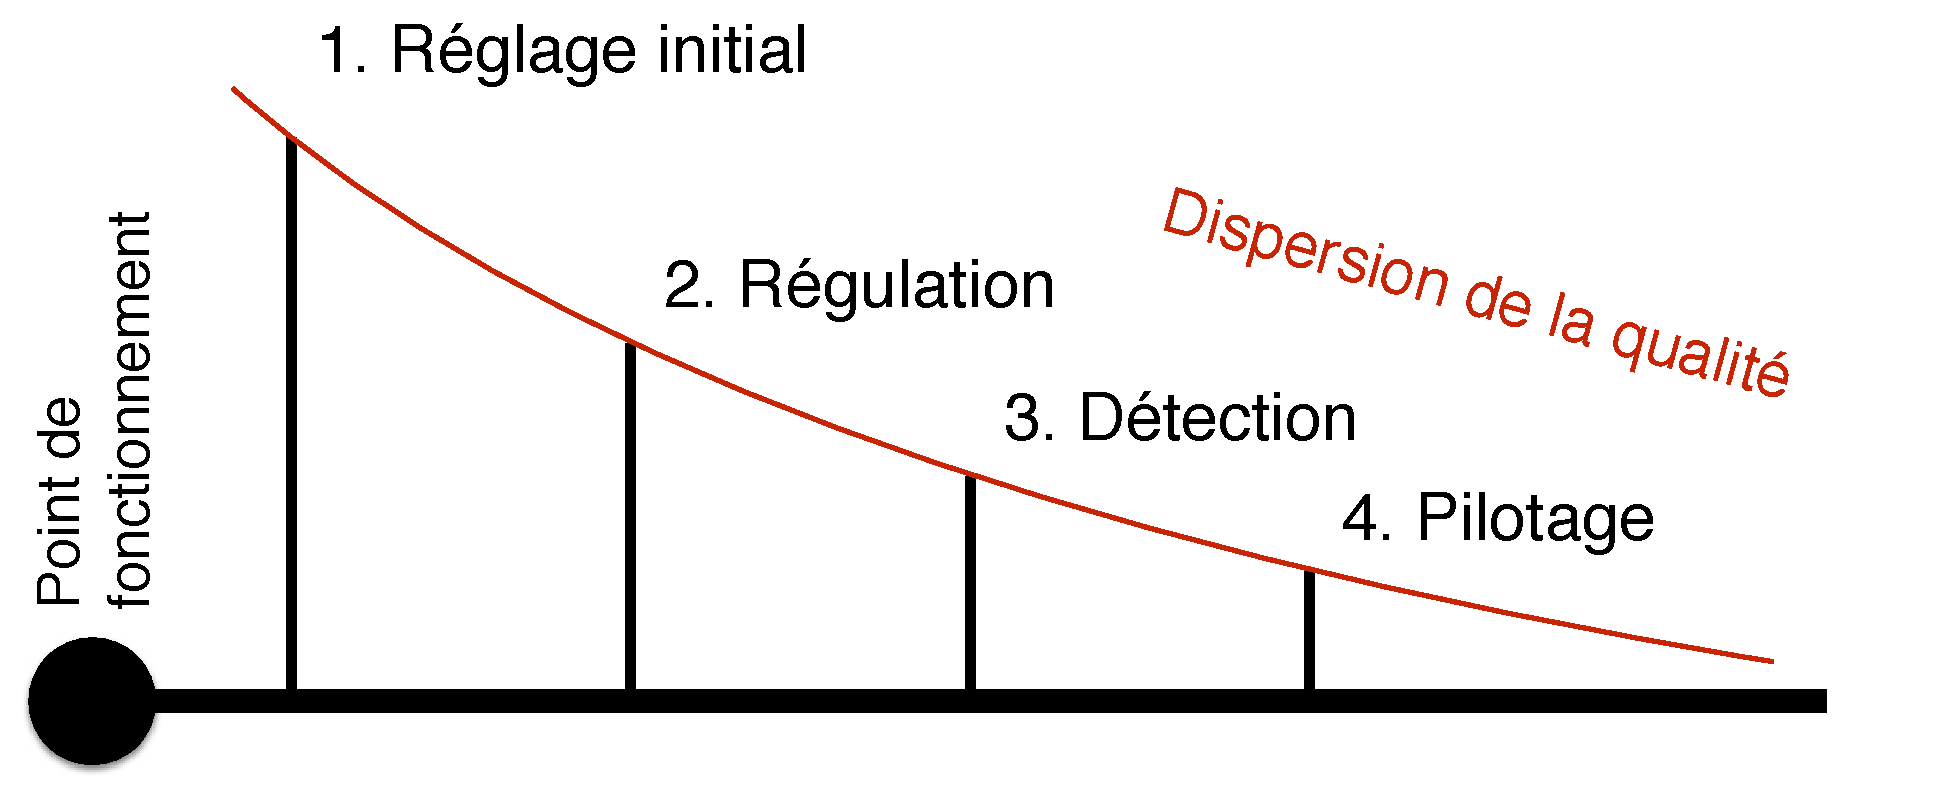
\includegraphics[width=\textwidth,height=\textheight,keepaspectratio]{../Chap1/Figures/Sapristi_EtatArt_Pilotage_en_Injection_Plastique.pdf}
%	\caption{Vers le pilotage du point de fonctionnement du procédé pour optimiser la qualité du produit.}
%	\label{fig:vers_le_pilotage}
%\end{figure}
% La Figure \ref{fig:vers_le_pilotage} récapitule cette démarche.


\section{Pilotage des caractéristiques de la pièce produite}
Le pilotage d’un procédé demande dans un premier temps de détecter les situations hors-contrôles.
Dans le cas où le procédé n'est pas dans sa configuration cible, on mesure l’écart entre la situation hors-contrôle et la situation cible.
Puis on ajuste un ou plusieurs paramètres réglables du procédé, afin de se rapprocher de la situation cible.
Plusieurs stratégies de pilotage ont été proposées dans la littérature.
Certaines utilise une modélisation physique simplifié du procédé, d'autres s'appuient sur une base de connaissance préétablie ou utilisent une analyse statistique.
Ces systèmes reposent sur l’instrumentation de la presse et de l'outillage pour mesurer les conditions appliquées au polymère.
L'évaluation des performances de ces stratégies passe par la mesure de dispersions des caractéristiques des produits.
Dans une démarche pragmatique, le pilotage des caractéristiques du produit peut également se réaliser en mesurant directement les caractéristiques des produits ($\boldsymbol{C_1}$ et $\boldsymbol{C_0}$ Figure \ref{fig:annexe_zigzag}).
% C'est l'objectif du projet FUI SAPRISTI.
Dans le cadre de nos travaux, nous mesurerons la qualité des pièces juste après la sortie de l'outillage ($\boldsymbol{C_1}$).
Notre démarche de mesure est présentée dans le Chapitre \ref{ch:measure}.

En 2001, \citeauthor{nwokah_control_2001} synthétisent les avancées réalisées dans le cadre du pilotage du procédé \cite{nwokah_control_2001}.
Ils définissent deux contraintes principales au développement du pilotage :
\begin{itemize}
	\item la méconnaissance des relations entre les paramètres d’entrées et les caractéristiques finales du produit ($\boldsymbol{P_i}$ et $\boldsymbol{C_i}$ Figure \ref{fig:annexe_zigzag}),
	\item le manque de possibilité d’ajustement des réglages du procédé.
\end{itemize}
Ils argumentent que l’amélioration d’une caractéristique du produit se fera souvent au détriment d’une autre caractéristique, ou bien par l'augmentation des coûts de produit.
Cette contrainte de coût est courante pour les productions industrielles à faible marge.

% \paragraph{Ajustement du procédé à partir des caractéristiques du produit}\mbox{} \\
L’ajustement statistique des procédés (\textit{Statistical Process Adjustement}) est un domaine situé à l’intersection de la régulation automatique et de la Maîtrise Statistique des Procédés.
Ce domaine d'étude étudie les relations entre les paramètres du procédé et les caractéristiques du produit, par une approche statistique.
Un exemple de relations entre les paramètres du procédé d’injection-moulage, qui conditionnent les caractéristiques de la pièce produite, concerne la vitesse d'avance ($\boldsymbol{P_3}$ Figure \ref{fig:annexe_zigzag}).
Celle-ci est liée à la viscosité de la matière ($\boldsymbol{C_3}$) et elle définit le débit d’injection ($\boldsymbol{P_3}$).

Il y a également une influence des paramètres du procédés sur la structure interne de la pièce.
Les travaux de doctorat de \citeauthor{giroud_mesure_2001} étudie l'influence des paramètres du procédé ($\boldsymbol{P_3}$) sur les contraintes internes ($\boldsymbol{C_1}$) \cite{giroud_mesure_2001}.
Le profil de pression appliqué à la pièce pendant la phase d'injection conditionne les contraintes internes résiduelles.
Ces contraintes seront figées dans la pièce par la modification de la forme et de l'orientation des chaînes de polymères.
La relaxation de ces contraintes peut provoquer des déformations géométriques.
C'est une des causes principales du retrait, qui apparait plusieurs heures après la production.

% \citeauthor{del_castillo_statistical_2006} réalise une rétrospective des travaux réalisés dans le domaine de l'Ajustement Statistique des Procédés \cite{del_castillo_statistical_2006}.
% Il identifie les méthodes de modélisation bayésiennes pour l'ajustement optimal des paramètres, comme des pistes privilégiées de recherche.
% Nous présenterons ces méthodes d'optimisations dans le Chapitre \ref{ch:metric_learning} §\ref{subsec:bayesian_opt}.

\subsection{Ajustement du procédé à partir de caractéristiques prédites} \label{parag:adjust_predict}
Il est difficile de mesurer les pièces en sortie de machine.
Les causes sont une durée de mesurage trop longue qui est supérieure au temps de cycle, un coût trop élevé ou simplement une mesure non faisable.
% De plus, le manque de spécifications concernant les caractéristiques de la qualité des pièces n’a pas encouragé l’utilisation de la mesure directe.
Excepté pour le dimensionnel, la notion de qualité dans les cahiers des charges est rarement normalisée.
Elle nécessite l'interprétation humaine, qui est difficile à programmer dans un ordinateur et également à transmettre entre humains.
Le transfert de la notion de qualité de l'expert humain vers le système de contrôle est un des objectifs de notre travail que nous présentons dans le Chapitre \ref{sec:metric_learning}).
C'est pourquoi de nombreux systèmes de la littérature ont choisi de prédire les caractéristiques des pièces produites ($\boldsymbol{C_1}$ Figure \ref{fig:annexe_zigzag}) à partir de variables du procédé ($\boldsymbol{P_i}$).
La prédiction obtenue est ensuite utilisée à des fins d’ajustement des paramètres du procédé pour optimiser les caractéristiques du produit.

En 1993, \citeauthor{haeussler_quality_1993} \cite{haeussler_quality_1993} utilisent un réseau de neurones pour prédire la masse et la longueur des pièces ($\boldsymbol{C_1}$ Figure \ref{fig:annexe_zigzag}), à partir de paramètres du procédé ($\boldsymbol{P_3}$, $\boldsymbol{P_2}$).
% Ils entrainent un réseau 9-21-2 à partir des mesures sur une production de 162 cycles continues.
Le réseau prédit la masse des pièces avec 20\% d'erreur et la longueur avec 11,6\% d'erreur.
Ces résultats sont comparés avec une régression polynomiale d'ordre 3, 25\% d'erreur pour la masse et 21\% d'erreur pour la longueur.
Le réseau de neurones est plus performant que la régression polynomiale d'ordre 3 car c'est une composée de fonctions non-linéaires.
% Cette étude conclut sur la nécessité de l'utilisation d'modèle adaptatif pour un réaliser le pilotage en cycle industriel.
Enfin, les auteurs remarquent que le modèle prédictif doit être enrichit au fur et à mesure des cycles, à partir des nouvelles mesures.
Le modèle ne doit pas se limiter à modéliser un jeu de données statique.
Nous reprenons cette idée dans nos travaux, en proposant un modèle de la notion de qualité qui est enrichit au fur et à mesure de la production §\ref{sec:metric_learning}.

En 1996, \citeauthor{woll_online_1996} proposent d'utiliser un réseau de neurones pour prédire la masse des pièces, à partir des profils de pression mesurées dans l'outillage et dans la buse \cite{woll_online_1996}.
À partir de la prédiction de la masse, la pièce est acceptée ou rebutée si la masse prédite est trop éloignée de la masse cible.
L'écart acceptable à la cible est définie selon la démarche MSP §\ref{parag:spc}.
Le réseau de neurones est appris comme un modèle inverse du procédé.
Les profils de pression sont les variables d'entrées ($\boldsymbol{C_2}$, $\boldsymbol{C_1}$ Figure \ref{fig:annexe_zigzag}) et les variables de sorties sont les consignes de pression de maintien ou de température du fourreau ($\boldsymbol{P_2, P_1}$).
Les paramètres sont ajustés cycle après cycle en comparant le profil de pression courant, avec le profil cible.
% L'analyse MSP est réalisée sur la valeur de pression maximale qui est mesurée dans l'outillage.
Le réseau est entrainé sur un jeu de données issues de simulations, afin d'éviter de réaliser une longue campagne d'essais.
% La convergence du modèle étant observé pour 2000 essais.
L'essai est réalisé pour un unique matériau et la caractéristique cible de la pièce est sa longueur.
% Les résultats montrent la capacité supérieure des réseaux de neurones à prédire les non linéarités comparée à la régression linéaire multiple utilisé par SPC.
% L'exactitude de la prédiction des mesures est augmentée de 10\% et le taux de faux positif est réduit de moitié.
% Le réseau rejette les perturbations.
% L'étude conclue sur la nécessité d'entrainer le réseau sur plusieurs profils dont les températures.
À contrario de cette étude, dans nos travaux, nous avons choisi de mesurer des données réelles sur des machines industrielles.
En effet, notre étude de la littérature montre que les simulations du procédé d'injection-moulage sont limitées.

Dans sa thèse, \citeauthor{chen_study_2002} proposent une méthodologie pour établir le profil de vitesse d’injection optimal ($\boldsymbol{P_3}$ Figure \ref{fig:zigzag}) \cite{chen_study_2002}.
Il modélise également la température du fondu par un second réseau de neurones ($\boldsymbol{P_2}$).
Disposant d'un modèle représentatif, il calcule le profil de température et la pression à imposer pour la phase de plastification, afin d'obtenir un température définie pour la matière qui sort de la buse ($\boldsymbol{C_3}$). 
% Il conclut sur la nécessité de garantir une vitesse de front constante lors de l'injection, afin d’obtenir une qualité produit optimale.

En 2004, dans ces travaux de doctorat, \citeauthor{yang_injection_2004} introduit l'utilisation du contrôle prédictif pour ajuster la vitesse d'avance de la vis lors de l'injection \cite{yang_injection_2004}.
Le contrôleur s'appuie sur l'automatique pour la régulation des procédés industriels (aussi appelée \textit{Global Process Control} ou \textit{Engineering Process Control}) qui consiste à utiliser des régulateurs Proportionnels Intégrateur Dérivateurs pour ajuster les paramètres afin d'obtenir des caractéristiques cibles du produit.
La masse de chaque pièce est prédite à partir des mesures sur le procédé ($\boldsymbol{C_2, C_1}$ Figure \ref{fig:annexe_zigzag}).
À partir de la prédiction, la vitesse d'injection ($\boldsymbol{P_3}$) est ajustée cycle après cycle.
% Un algorithme d'apprentissage itératif en logique floue compense les temps de réponses long des actionneurs.
Ce travail montre la limite que pose l'utilisation des servovalves pour ajuster les paramètres du procédé.
Les servovalves ont un temps de réponse lent, de l'ordre de la seconde.
Ainsi, il est nécessaire d'anticiper la valeur de la consigne.  %, notamment lorsqu'il s'agit d'imposer des consignes temporelles précises.
% À l'aide de l'ensemble des ces techniques, ce travail montre qu'il est possible de détecter les variations de la masse pendant le cycle, sans nécessité une pesée de la pièce.
Ce travail montre qu'il est possible d'ajuster les conditions de maintien et de refroidissement afin de compenser la variation de masse prédite.
L'auteur conclut sur la possibilité de piloter d'autres caractéristiques du produits, en utilisant la même démarche : les géométries et l'aspect des pièces pourraient être ajustés, sous réserve de pouvoir prédire les caractéristiques.

\subsection{Ajustement à partir des caractéristiques mesurées sur le produit}
La section précédentes étudiaient la prédiction des caractéristiques des produits.
Il est également possible de mesurer les caractéristiques du produit.
Dans l'ensemble de la littérature, les caractéristiques mesurées sur les pièces sont limitées à la masse et à quelques cotations géométriques.
L'aspect des pièces n'a jamais été mesurée en cycle.
La masse est la caractéristique la plus mesurée, car la pesée peut facilement être réalisée pendant le cycle d'injection-moulage.
Il suffit de disposer d'un bras robotique préhenseur et d'une balance instrumentée.
Les mesures complémentaires de la qualité des produits sont effectuées après de la production d'un lot, mais non pendant le cycle d'injection.
Il serait intéressant de réaliser une caractérisation complète de la pièce produite, pendant le temps de cycle, afin de pouvoir optimiser les caractéristiques des pièces suivantes, à partir de ces mesures.
La limite à cette démarche est la durée des mesures, qui doit être inférieure au temps de cycle.

En 1998, \citeauthor{fournier_conduite_2006} a proposé un ajustement des paramètres du procédé à partir de la mesure de la masse du produit \cite{fournier_conduite_2006}.
Le matériau qui a été utilisé est le Poly(Téréphtalate de Butylène).
C'est un semi-cristallin sensible aux phénomènes de retrait.
Le système de l'étude utilise un modèle physique simplifié du procédé pour réguler les paramètres en boucle fermé.
% L'écart entre la masse mesurée et la masse cible est ajouté à la boucle de régulation.
Deux perturbations ont été appliquées pendant le cycle : un changement de la matière et un changement de la température dans le fourreau.
Afin de limiter les contraintes internes du matériau, les pièces sont passées par un recuit.
Les mesures des retraits volumiques et de résiliences (chocs Charpy) ont montré une dispersion de masse réduite de 24\% avec l'utilisation du correcteur sur la masse.
La dispersion du retrait volumique, mesurée deux jours après la production des pièces, est réduite de moitié.
Cependant, une cotation géométrique augmente ; elle correspond à l'épaisseur de la pièce.
Après recuit, le retrait volumique est diminué de 12\% par rapport à un procédé non régulé.
La résilience après recuit est quant à elle augmentée de 23\%.
% L'étape de recuit peut être assimilé aux étapes de peintures qu'une pièce est susceptible de subir.
Ces résultats obtenus sont encourageants.
% L'étude montre qu'il y a un intérêt à ajuster les paramètres du procédé en fonction des caractéristiques du produit mesurées dès la sortie de la machine ($\boldsymbol{P_1}$).
% Nos travaux s'inscrivent dans cette démarche.

Une piste de travail importante serait de considérer les caractéristiques des produits finaux ($\boldsymbol{C_0}$ Figure \ref{fig:annexe_zigzag}) pour ajuster le procédé.
Cela nécessitera nécessairement l'utilisation d'un modèle prédictif, car la pièce finale sera obtenue plusieurs heures après son moulage, après son refroidissement.

La même année, \citeauthor{ivester_automatic_1998} ont proposé une méthode d'ajustement à partir de la mesure des caractéristiques \cite{ivester_automatic_1998}.  % qui s'appuie sur un modèle du procédé qui est construit au fur et à mesure de la production,
Les paramètres du procédé sont ajustés par descente de gradient au fur et à mesure de la production (cette méthode est détaillée dans le Chapitre \ref{ch:metric_learning} \ref{parag:neural_networks}).
% Ainsi, le modèle procédé n’est mis à jour que lorsqu’il ne permet plus d’estimer les changements.
L'étude indique que la caractérisation de la qualité des pièces est réalisée par un opérateur humain.
Dans le cadre de nos travaux, nous chercherons à automatiser cette caractérisation.
% Cette méthode d’optimisation des réglages requière que l’opérateur entre les paramètres mesurées ou analyse les mesures dans le cas de caractéristiques d’aspect.
% L’étude conclue sur la viabilité de la méthode et sur l’intérêt d’automatiser la mesure de la qualité des pièces.
Cette méthode est néanmoins dépendante des points de fonctionnement initiaux, qui sont choisis aléatoirement.
C’est pourquoi, \citeauthor{yang_knowledgebased_2000} propose l'ajustement des paramètres du procédé par optimisation d'un modèle qui lie les paramètres avec les caractéristiques du produit, préalablement établi \cite{yang_knowledgebased_2000}.
% C’est un modèle multivarié qui permet de rendre indépendant le système des paramètres initiaux avant optimisation.
Un modèle initial multivarié est définie à partir de la connaissance théorique du procédé.
% C’est ce modèle empirique multivarié qui détermine le point de fonctionnement initial.
% Un algorithme d'apprentissage permet d’optimiser ce modèle pour un produit et une machine.
% L’intérêt du modèle préétablie est de proposer un point de fonctionnement.
% L'apprentissage passe par la comparaison des caractéristiques qualités données par le modèle préétablie et des caractéristiques qualités mesurées sur les pièces.
% Par la suite, le modèle initial est ajusté au fur et à mesure de la production.
Par la suite, les caractéristiques prédites par le modèle sont comparées aux mesures réelles, et les coefficients du modèle sont ajustés pour diminuer l'écart de la prédiction.
% L'étude compare la faisabilité théorique obtenue par simulation et le point de fonctionnement donné par le modèle relationnel KBT, puis le point de fonctionnement obtenu par plan d'expérience central composite.
Une comparaison expérimentale est réalisée entre le système proposé et un point de fonctionnement optimisé à partir de la réalisation d'un plan d'expériences Central Composite (§\ref{parag:doe_cc}).
7 caractéristiques qualités sont mesurées sur le produit.
5 paramètres sont pilotés sur la machine.  % et leurs limites sont connues du modèle.
Le protocole expérimental est détaillé : les 20 premières pièces de chaque essai ne sont pas prises en compte, en attendant la stabilisation du procédé.
Par la suite, 5 pièces sont mesurées 15 à 25 minutes\footnote{
	Nous remarquons que l'amplitude temporelle de 10 minutes est grande.
	En effet, si les pièces sont conservées dans le même atelier de production, alors nous pouvons estimer que leur vitesse de refroidissement est identique.
	Aussi pour une même durée de refroidissement, les caractéristiques seront identiques.
	Or cette durée de refroidissement varie ici beaucoup. 
	Nous recommandons de mesurer les pièces quelques secondes après la sortie du moule, en maitrisant le délai de mesure, afin d'éviter d'introduire une erreur.} après leur sortie du moule pour que leurs caractéristiques géométriques soient également stabilisées.
Les résultats de l'étude montrent que le plan Central Composite n'inclue qu'un petit espace de la plage de réglage du procédé.
Il est alors difficile de trouver un point de fonctionnement optimal à partir du modèle issu du plan d’expérience.
L'étude aurait pû positionner les bornes du plan d'expériences aux limites du procédé.
Le système d'apprentissage proposé dans l'étude est capable de trouver un point de fonctionnement satisfaisant en 10 essais, tandis que le plan Central Composite demande 45 essais.
L'introduction d'un modèle initial issue de la connaissance théorique du procédé permet de diminuer le nombre d'essais à réaliser pour trouver une solution optimale.
% Enfin, nous notons que la mesure des caractéristiques qualités du produit est ici facilité car ce sont des disques DVD.
% Les mesures ont une résolution élevé puisqu'un micromètre laser mesure un profil sur la surface des disques.
% La capabilité du moyen de mesure est excellente.
% Une bonne capabilité du système de mesures est un pré-requis, pour la caractérisation des pièces, et pour le pilotage du procédé.

En 2001, \citeauthor{lau_neural_2001} propose de réaliser un modèle inverse du procédé, à multiples entrées et multiples sorties, par apprentissage d'un réseau de neurones \cite{lau_neural_2001}. % vérifier les capacités de création  d'un modèle multi entrées-sorties du procédé d'injection par réseau de neurones à propagation inverse.
L’objectif est que le réseau suggère des ajustements des paramètres du procédé pour obtenir une pièce cible aux dimensions spécifiées.
Les caractéristiques dimensionnelles portent sur trois longueurs et l'épaisseur de la pièce.
L'apprentissage du réseau est réalisé sur les mesures récoltés sur 100 pièces, en faisant varier sept paramètres du procédé : la température du fourreau centrale et la température de l'arrière du fourreau, la vitesse de fermeture de l’outillage, la vitesse d’avance de la vis, la force de fermeture, la durée d'injection, la durée de refroidissement, la vitesse d'avance de la vis lors de l'injection et la pression d'injection.
% L'étude mentionne que les quatre dimensions étudiées n'ont pas les mêmes valeurs en fonction de la journées de réalisation des essais.  %, malgré la répétition de paramètres identiques, 
% Il ne suffit pas de répéter des paramètres
Les valeurs des dimensions attendues sont appliquées en entrée du modèle.
Ce dernier indique en sortie les valeurs du point de fonctionnement permettant de produire une pièce avec ces dimensions.
La démarche du système est alors d'obtenir l'écart entre les paramètres pour les caractéristiques actuelles et pour les caractéristiques cibles, puis d'ajuster les paramètres en soustrayant ces écarts, afin de compenser les variations des caractéristiques pièces.
En connaissant le réglage utilisé pour produire les pièces, l'étude propose de régler les paramètres dans des proportions inverses afin de compenser les variations de pièces.
Cette démarche suppose que les paramètres sont indépendants, ce qui n'est pas le cas pour le procédé d'injection-moulage.
% Néanmoins, après 3 itérations de réglages successifs, le réseau parvient à converger vers une erreur quadratique moyenne (RMS) de 0,07.
% Ce résultat est comparé à une précédente étude des auteurs [Lau et Wong, 1998] qui utilisait un système hybride à logique floue qui convergeait en 3 itérations vers une erreur quadratique moyenne (RMS) de 0,06.
% La méthode proposée est moins performante qu'un système à logique flou et réseaux de neurones mais plus simple à mettre en œuvre.
% De plus, une optimisation de la topologie du réseau de neurones, telle que la recherche en informatique la permet aujourd'hui améliorerait ce résultat.

Récemment, en 2015, \cite{johnston_-line_2015} réalise une étude à l'aide d'un plan d'expériences à quinze essais pour douze facteurs, pendant 30 minutes de production par essais, totalisant 942 cycles d'injection-moulage, soit 60 pièces par essais.
% Il dérive des fonctions de transfert et des composantes principales pour chacune des 46 sorties du procédé.
Pour chaque cycle, une boucle d'optimisation évalue et minimise l'écart à une dimension géométrique cible par un ajustement des paramètres du procédés ($\boldsymbol{P_1, P_2, P_3}$ Figure \ref{fig:annexe_zigzag}).
% Le contrôleur qui est proposé est capable de détecter les variations du procédé par comparaison avec un modèle de référence préétabli.
% Le contrôleur ajuste alors les paramètres pour atteindre le modèle de référence.
Un objectif de réduction du temps de cycle est ajouté grâce à une pénalité temporelle dans la fonction à minimiser.
Un double objectif est atteint : le temps de cycle est réduit et la variabilité des dimensions des pièces est réduite.
L'étude conclut qu’une optimisation  multi-paramètres, par exemple sur les caractéristiques dimensionnelles, est possible.
Les auteurs mettent en valeur l'intérêt de leur méthode par rapport à un ajustement manuel des paramètres du procédé.
Leur système permet de réduire le nombre d'essais à réaliser pour régler le procédé d'un facteur dix.




\FloatBarrier
\chapter{Annexe 2 : Titre}
\label{Ann:2}

%==============================================================================	Résumé du chapitre

\begin{center}
\rule{0.7\linewidth}{.5pt}
\begin{minipage}{0.7\linewidth}
\smallskip

\textit{Résumé ici.
}

%\smallskip
\end{minipage}
\smallskip
\rule{0.7\linewidth}{.5pt}
\end{center}

\minitoc
\newpage


\section{Section 1}
\subsection{Sous section 1}
\blindtext
\subsection{Sous section 2}
\blindtext



\FloatBarrier
\chapter{Annexe 3 : Titre}
\label{Ann:3}

%==============================================================================	Résumé du chapitre

\begin{center}
\rule{0.7\linewidth}{.5pt}
\begin{minipage}{0.7\linewidth}
\smallskip

\textit{Résumé ici.
}

%\smallskip
\end{minipage}
\smallskip
\rule{0.7\linewidth}{.5pt}
\end{center}

\minitoc
\newpage

\section{Section 1}
\subsection{Sous section 1}
\blindtext
\subsection{Sous section 2}
\blindtext



